\documentclass[10pt,b5paper]{ltjsarticle}

\usepackage[margin=15truemm, top=5truemm, bottom=5truemm]{geometry}

\usepackage{amsmath}
\usepackage{amssymb}
\pagestyle{empty}


\usepackage{graphicx}	% required for `\includegraphics' (yatex added)
\usepackage{url}	% required for `\url' (yatex added)

\usepackage{listings}
%\usepackage{jvlisting}
%ここからソースコードの表示に関する設定
%\lstset{
%  basicstyle={\ttfamily},
%  identifierstyle={\small},
%  commentstyle={\smallitshape},
%  keywordstyle={\small\bfseries},
%  ndkeywordstyle={\small},
%  stringstyle={\small\ttfamily},
%  frame={tb},
%  breaklines=true,
%  columns=[l]{fullflexible},
%  numbers=left,
%  xrightmargin=0zw,
%  xleftmargin=3zw,
%  numberstyle={\scriptsize},
%  stepnumber=1,
%  numbersep=1zw,
%  lineskip=-0.5ex
%}
%ここまでソースコードの表示に関する設定




\begin{document}


円$C: x^2+y^2=1$
と
直線$l:y=ax-2a$
の交点

円の式に直線の式を代入すると
次の式が得られる。
\begin{equation}
 (a^2+1)x^2-4a^2x+4a^2-1=0
\end{equation}
この代入は円の式が変形されただけではなく、
$\mathbb{R}^2$全体の変換を行っている
と考える。

次の写像$f$が変換写像。
\begin{equation}
 f: \qquad \mathbb{R}^2 \rightarrow \mathbb{R}^2
 (x,y) \mapsto (X,Y)=(x,y-ax+2a)
  \qquad
\end{equation}
写像の定義域を$A=\mathbb{R}^2$、値域を$B=\mathbb{R}^2$と呼ぶことにする。
$A$は$xy$平面、$B$は$XY$平面。

$y=ax-2a$を変形して$y-ax+2a=0$となる。
$y=ax-2a$を代入するという事は
$y$と$ax-2a$が等しい世界であり、
これは$y-ax+2a$が$0$となる世界のことを指す。
$A$の直線$l$は$y=ax-2a$を満たすので、
$y-ax+2a=0$を満たす点の集まりである。
$B$では$Y=y-ax+2a=0$である為、$X$軸と重なる。
つまり、写像$f$で$A$の直線$l$は$B$の$X$軸に対応する。

$A$では$C$は円、$l$は直線であるが、
写像$f$にて変換された$B$では
$l$が$X$軸になっている。
$C$は$B$では
$(a^2+1)X^2+(2aY-4a^2)X+Y^2-4aY+4a^2-1=0$
で表される楕円になる。

%具体的に考える。

\hrulefill

$a=1$の場合
\quad
左:$A$ $xy$平面
\hfil
右:$B$ $XY$平面
\begin{center}
 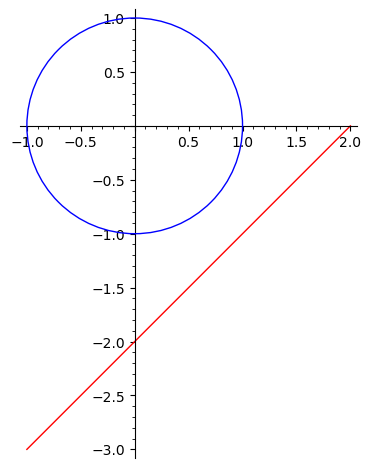
\includegraphics[scale=0.6]{tra.png}
\hfill % $\rightarrow$
 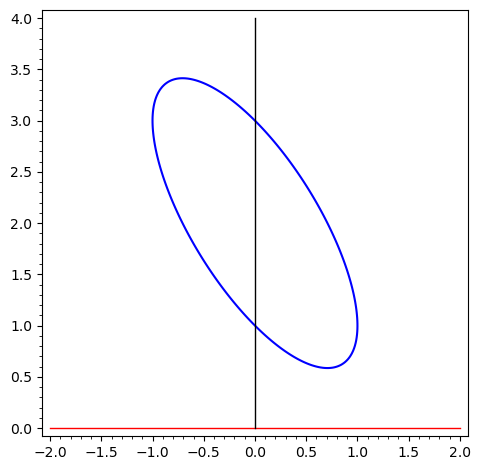
\includegraphics[scale=0.6]{trb.png}
\end{center}

\dotfill

$a=\frac{1}{2}$の場合
\quad
左:$A$ $xy$平面
\hfil
右:$B$ $XY$平面
\begin{center}
 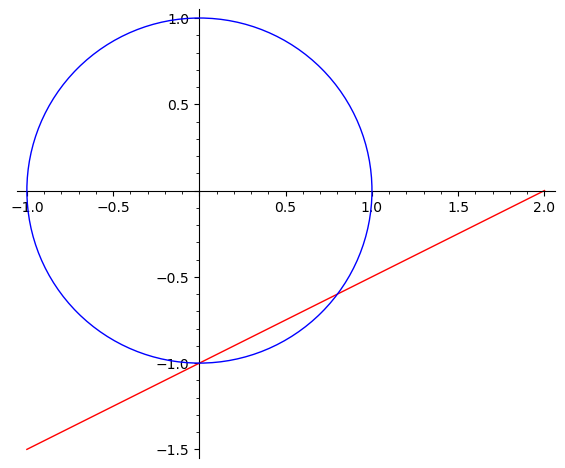
\includegraphics[scale=0.5]{tra_h.png}
\hfill % $\rightarrow$
 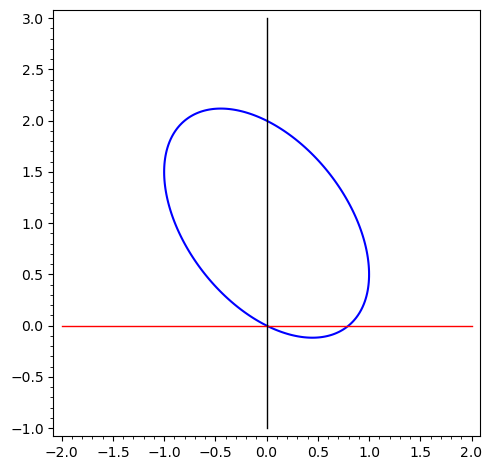
\includegraphics[scale=0.5]{trb_h.png}
\end{center}

\hrulefill

$A$の円$C$と直線$l$との交点は
$B$の楕円と$X$軸の交点として現れる。
$f$の逆写像$f^{-1}$が存在し、
$B$での交点は$A$でも交点となる為、
$B$での交点を考えるだけでよい。
\begin{equation}
 f^{-1}: B(=\mathbb{R}^2) \rightarrow A(=\mathbb{R}^2)
  \quad
  (X,Y) \mapsto (x,y)=(X,Y+aX-2a)
\end{equation}

$B$での交点を求めるために、
$X$軸の式$Y=0$を楕円の式に代入すると
最初の式
$(a^2+1)x^2-4a^2x+4a^2-1=0$
が得られる。
これを解くと$x$の値が求まるが、
$f$の定義から$A$でも$B$でも同じ値が交点の$x$座標であり、
値の範囲は$-1\leq x\leq 1 \ (-1\leq X\leq 1)$となる。

これにより、
$x^2+y^2=1$と$y=ax-2a$の交点の$x$座標は
方程式$(a^2+1)x^2-4a^2x+4a^2-1=0$の解と対応している。




\hrulefill

グラフの式 sagemath

\url{https://sagecell.sagemath.org/}

\dotfill

\begin{lstlisting}[language=Python,basicstyle={\scriptsize}]
a=1

c=circle((0,0), 1)
l=plot(a*(x-2),[x,-1,2],color='red')
show(c+l,aspect_ratio=1)

var('x,y')
b=implicit_plot((a^2+1)*x^2+(2*a*y-4*a^2)*x+y^2-4*a*y+4*a^2-1,[x,-1,1],[y,0,4])
xax=line([(-2,0),(2,0)],color='red')
yax=line([(0,0),(0,4)],color='black')
show(b+xax+yax,aspect_ratio=1)

save(c+l,'tra.png', aspect_ratio=1)
save(b+xax+yax,'trb.png', aspect_ratio=1)
\end{lstlisting}

\dotfill

\begin{lstlisting}[language=Python,basicstyle={\scriptsize}]
a=1/2

c=circle((0,0), 1)
l=plot(a*(x-2),[x,-1,2],color='red')
show(c+l,aspect_ratio=1)

var('x,y')
b=implicit_plot((a^2+1)*x^2+(2*a*y-4*a^2)*x+y^2-4*a*y+4*a^2-1,[x,-1,1],[y,-1,3])
xax=line([(-2,0),(2,0)],color='red')
yax=line([(0,-1),(0,3)],color='black')
show(b+xax+yax,aspect_ratio=1)

save(c+l,'tra_h.png', aspect_ratio=1)
save(b+xax+yax,'trb_h.png', aspect_ratio=1)
\end{lstlisting}

\end{document}
